\chapter{Judges, Costs and the Justice System}
\label{ch:systemcosts}

\section{Justice is a scarce resource}

Courts cost money. Judges are paid, court buildings maintained, staff employed, records kept. Parties pay lawyers and experts, and they and their witnesses give up time. Delay imposes further costs: a claimant waiting for compensation, a business with capital tied up, an accused person on remand. Every hour a judge spends on one case is an hour not spent on another. A legal system is therefore an allocation problem: how to spend limited resources to produce the most justice. This chapter applies the decision theory of Chapter~\ref{ch:decisions} to that problem. It asks how much accuracy is worth, how judges' time should be allocated, what appeals are for, and how the rules on legal costs shape the cases that reach court.\index{costs of justice}

\section{The value of accuracy}

\subsection{Kaplow's question}

Louis Kaplow asked why the legal system should value accuracy at all \citep{kaplow1994}. On Kaplow's view, accuracy in adjudication has no value in itself; its value lies in its effects. Accurate determinations of liability improve incentives, because people who know they will be held liable only if they cause harm, and will be held liable if they do, take appropriate care. Accurate determinations of damages improve incentives in the same way. Accuracy also matters for fairness and for the legitimacy of the courts. But each of these benefits has limits, and accuracy is costly. The optimal level of accuracy balances its marginal benefit against its marginal cost.\index{Kaplow, Louis}\index{accuracy, value of}

\subsection{The trade off}

Figure~\ref{fig:accuracy} shows the trade off for a single case. As resources devoted to the case increase, the cost of process rises and the expected cost of errors falls, quickly at first and then more slowly. Total cost is minimised where the marginal cost of process equals the marginal reduction in error cost. The optimum depends on the stakes. A case where an error would cost a great deal (a murder trial, a dispute over a large business) justifies more process; a small claim justifies less. This is why legal systems have tracks: small claims procedures, fast, intermediate and multi tracks in England, magistrates' courts and the Crown Court, summary and plenary procedures elsewhere. Each track is a point on the trade off appropriate to a class of cases.

\begin{figure}[t]
\centering
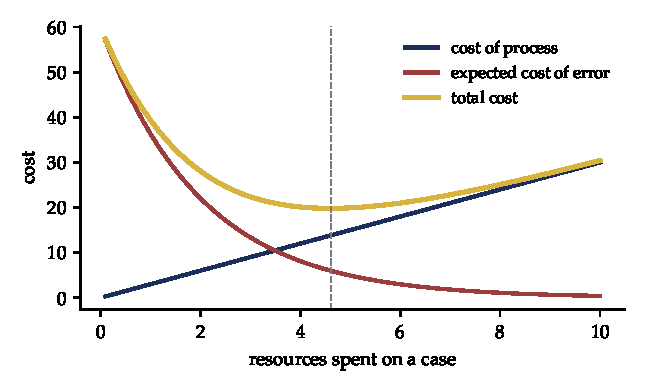
\includegraphics[width=\linewidth]{fig_accuracy}
\caption{The cost of process, the expected cost of error and their sum, as functions of the resources spent on a case. The dashed line marks the optimum. Illustrative.}
\label{fig:accuracy}
\end{figure}

\subsection{Accuracy about what?}

Kaplow emphasised that the value of accuracy differs across issues. Accuracy about whether a defendant was negligent matters for incentives because it determines whether careless people pay; accuracy about the exact amount of damages matters less if errors are unbiased, since risk-neutral potential defendants care about expected liability, and matters only to the extent that they can foresee the harm they might cause when choosing precautions \citep{kaplowshavell1996}. Courts might therefore spend more on liability and less on quantum, or use rough schedules for damages in routine cases, such as the tariffs for injuries in the Judicial College guidelines in England, while reserving full assessment for large claims.

\section{Allocating judges' time}

\subsection{The docket as a portfolio}

A judge or a court has a docket of cases and a fixed amount of time. Each case would benefit from more time, in the sense of a lower expected error cost, but the benefit varies. The efficient allocation gives each case time until the marginal reduction in expected error cost per hour is equal across cases. Cases near the decision threshold, where the posterior is close to the standard of proof, benefit most from additional evidence and argument, as the value of information analysis of Chapter~\ref{ch:standards} showed. Cases far from the threshold benefit little and can be decided quickly.\index{docket management}

This principle supports active case management. Under the Civil Procedure Rules introduced after Lord Woolf's reforms, English courts must seek to give effect to the overriding objective\index{overriding objective} of dealing with cases justly and at proportionate cost, including by allotting to each case an appropriate share of the court's resources while taking into account the need to allot resources to other cases. The phrase is a statement of the allocation principle. A Bayesian approach would make it operational, by estimating for each case the probability of each outcome and the value of further process, and allocating time accordingly.

\subsection{Judges as a cost of the system}

Judges' time is the scarcest resource in most court systems. In England and Wales, shortages of judges and recorders have contributed to large backlogs in the Crown Court, with some trials listed long after charge. In India, as Chapter~\ref{ch:india} showed, the judge to population ratio is a fraction of what the Law Commission recommended. In the United States, judicial vacancies and rising caseloads have lengthened federal civil dockets. The marginal value of an additional judge is the value of the cases that judge would decide, plus the reduction in delay for all cases. Where delay is long, that value is large: each year of delay for a remanded defendant costs the defendant their liberty and the state the cost of custody, and each year of delay in a civil case reduces the value of the claim and of the incentive the law provides.

\subsection{The cost of delay}

The cost of delay can be estimated. For a civil claim of value $J$ with probability of success $p$, a delay of $t$ years at a discount rate $r$ reduces the present value of the expected recovery from $pJ$ to $pJ e^{-rt}$, and if interest awarded does not fully compensate for delay, the claimant bears the difference. Delay also reduces accuracy, as memories fade and evidence is lost, which raises the expected error cost. For a remanded defendant, the cost is the value of liberty lost, which the law recognises by crediting time on remand against any sentence, but which is not compensated if the defendant is acquitted. In a system with long delays, these costs can dwarf the direct costs of courts.

\section{Appeals as error correction}

Steven Shavell analysed appeals as a means of correcting errors \citep{shavell1995}. If trial courts make errors and appellate courts can detect some of them, an appeal system reduces the expected error cost at the price of appellate resources and further delay. Appeals are efficient when the parties who appeal are disproportionately those who suffered errors, so that the appellate courts' resources are concentrated on the cases most likely to be wrong. Parties have private information about whether the trial court erred, and the cost of appealing deters those with weak grounds; the appeal process works as a screen.\index{appeals}

In Bayesian terms, the decision to appeal is a decision under uncertainty about the appellate outcome, and the permission stage, which requires a real prospect of success or some other compelling reason in England, is a threshold on that probability. Permission to appeal economises on appellate time by excluding appeals with low posterior probability of success. The threshold should depend on the stakes and on the value of the appeal for clarifying the law, since appellate decisions are public goods that guide future cases. A case with a modest probability of success but a large question of law may warrant permission because of its value as precedent, a benefit that accrues to people other than the parties.

\section{Who pays: costs rules}

\subsection{The English and American rules}

Under the English rule the losing party pays the winner's reasonable costs, assessed by the court. Under the American rule each party bears its own costs, subject to exceptions. Chapter~\ref{ch:becker} discussed how these rules affect settlement. Here we consider their effect on access and on the composition of cases. The English rule raises the stakes of litigation, deterring claims with a low probability of success, since a losing claimant pays two sets of costs, and encouraging claims with a high probability, since a winning claimant recovers most of its costs. The American rule makes small claims with a high probability of success uneconomic, since the claimant's costs eat into the recovery, and allows weak claims with large stakes to be brought, since the defendant cannot recover its costs.\index{costs rules}

\subsection{Proportionality and costs management}

In England, Lord Justice Jackson's review of civil litigation costs led to reforms in 2013 that made proportionality a central test for recoverable costs, introduced costs budgeting, under which the court approves each party's budget in advance, and changed the rules on conditional fee agreements and after the event insurance. From October 2023 fixed recoverable costs\index{fixed recoverable costs} were extended to most civil claims of up to one hundred thousand pounds. These reforms implement the principle that the cost of process should be proportionate to what is at stake, the principle illustrated in Figure~\ref{fig:accuracy}.

Fixed costs trade accuracy for predictability. A party knows in advance what it will recover or pay if it wins or loses, which makes the expected value calculations of Chapter~\ref{ch:decisions} easier and settlement more likely. The cost is that cases requiring more work than the fixed amount allows may be under resourced. The decision theoretic view supports fixed costs for routine cases with predictable demands and budgeted costs for complex ones, the structure the English reforms adopted.

\subsection{Legal aid}

When one party cannot afford representation, the adversarial system of Chapter~\ref{ch:commoncivil} loses its main safeguard: the fact finder hears only one side's evidence searched with vigour. Legal aid, by funding representation, restores the competition between information gatherers that makes adversarial procedure work. Cuts to civil legal aid\index{legal aid} in England under the Legal Aid, Sentencing and Punishment of Offenders Act 2012 led to a large increase in litigants in person, notably in family cases, who may take more court time per case and may be less able to present meritorious claims. The decision theoretic analysis suggests that the savings from legal aid cuts should be weighed against the increased error cost and the increased cost of court time, both of which fall on the system.

\section{Measuring the system}

A court system that wants to allocate resources well needs data: the number and type of cases, their duration, outcomes, appeals and reversals, and costs. Reversal rates on appeal are a rough measure of error, though they understate it, since most errors are not appealed and appellate courts defer to trial courts on findings of fact and reverse them only for clear error. Delay statistics measure one cost. Surveys of court users measure perceived fairness. The Indian National Judicial Data Grid of Chapter~\ref{ch:india} shows what public data on a court system can look like. A Bayesian court administrator would use such data to estimate the value of information and the cost of delay by case type, and allocate judges, courtrooms and support accordingly.

\section{Judges as decision makers}

Finally, judges are themselves decision makers with objectives and constraints. They seek to decide correctly, to avoid reversal, to manage their dockets, and in many systems to advance in their careers. Their incentives shape their decisions. Richard Posner, a judge as well as a scholar, wrote about judges as economic actors who maximise a utility that includes leisure, reputation and the satisfaction of deciding well. Research has documented effects of caseload pressure on decisions, and the noise between judges to which Chapter~\ref{ch:hume} returns. A system that measures judges' performance risks distorting it, as France feared when it banned judge analytics (Chapter~\ref{ch:commoncivil}); a system that does not measure it cannot improve it. The Bayesian response is to measure error and delay at the level of the court and the case type, where the purpose is allocation and reform, and to protect individual judges' independence in deciding the merits.

\section*{Notes and Questions}
\addcontentsline{toc}{section}{Notes and Questions}
\begin{enumerate}[label=\arabic*.]
\item In Figure~\ref{fig:accuracy}, the cost of process is $3e$ and the expected error cost $60e^{-0.5e}$. Find the optimal $e$. How does it change if the stakes, and hence the error cost, double?
\item A court has two kinds of case: those with posterior near one half, where an hour of hearing reduces expected error cost by ten units, and those with posterior near zero or one, where it reduces it by one unit. How should a judge with ten hours allocate time between five cases of each kind?
\item Compute the present value lost by a claimant with a fifty per cent chance of recovering one hundred thousand pounds if trial is delayed by two years at a discount rate of five per cent (continuous compounding) and interest is awarded at two per cent.
\item Explain Shavell's argument that appeals can be an inexpensive way to correct errors, because litigants' private knowledge of whether the trial court erred screens which cases reach the appellate court.
\item Under fixed recoverable costs, a claimant knows it will recover a fixed sum if it wins. How does this change the decision whether to sue, compared with assessed costs?
\item Should a court system publish statistics on the reversal rates of individual judges? Weigh the value of the information against its costs.
\end{enumerate}

\section*{Further reading}
Kaplow on the value of accuracy \citep{kaplow1994}; Shavell on appeals \citep{shavell1995}; and the reports of Lord Woolf and Lord Justice Jackson on civil justice in England and Wales.
